\epi{``I am interested in this and hope to do something.''}
{\textit{On adding complex numbers to Go}\\ \textsc{KEN THOMPSON}}

\noindent{}What is Go? From the website \cite{go_web}:
\begin{quote}
The Go programming language is an open source project to make
programmers more productive. Go is expressive, concise, clean, and
efficient. Its concurrency mechanisms make it easy to write programs
that get the most out of multi core and networked machines, while its
novel type system enables flexible and modular program construction. Go
compiles quickly to machine code yet has the convenience of garbage
collection and the power of run-time reflection. It's a fast, statically
typed, compiled language that feels like a dynamically typed,
interpreted language.
\end{quote}

Go 1 is the first stable release of the language Go. 
This document and all exercises work with Go 1 -- if not, it's a bug.

The following convention is used throughout this book:
\begin{itemize}
\item Code is displayed in \prog{DejaVu Mono};

\begin{figure}[H]
\caption{Chronology of Go}
\label{fig:chrono-of-go2}
\begin{center}
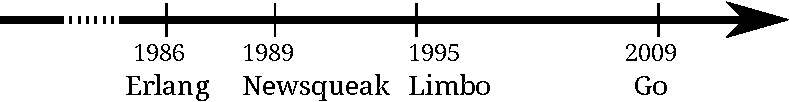
\includegraphics[scale=0.65]{fig/go-history.pdf}
\end{center}
\end{figure}

\section{Using DRBD and Heartbeat sync in GCE Zones}
\item Use \index{DRBD} to failover xymon data \key{DejaVu Mono Bold};

\begin{figure}[H]
\caption{DRBD in GCE to failover Xymon data}
\label{gce-xymon-failover-drbd}
\begin{center}
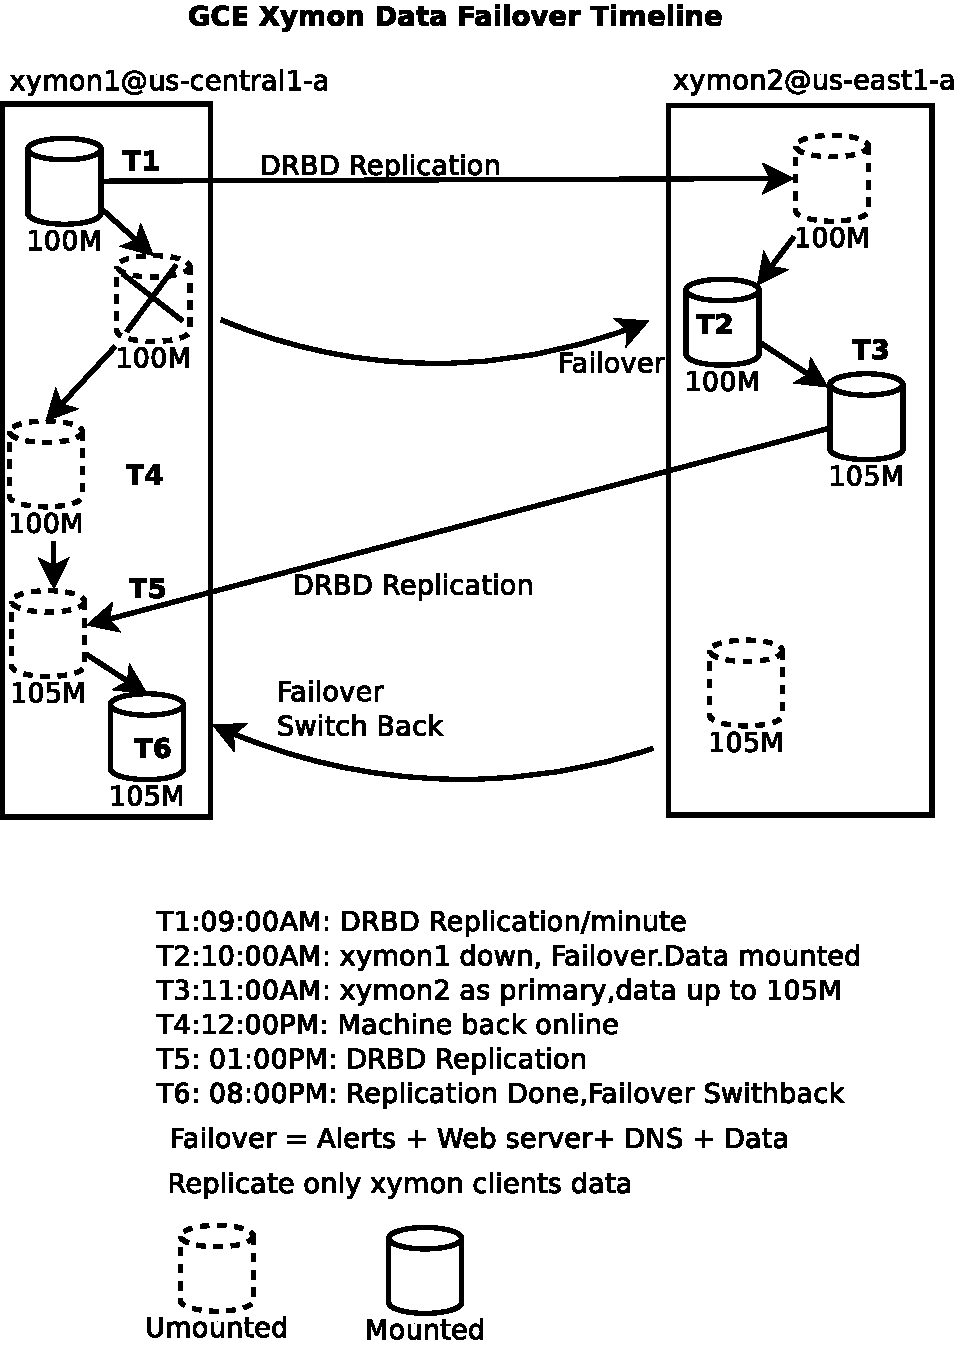
\includegraphics[scale=0.65]{dia/gce-xymon-failover-drbd.pdf}
\end{center}
\end{figure}

\item Comments are displayed in \rem{DejaVu Mono Italic};
\begin{figure}[H]
\caption{Two Nodes Loosely Cupled Cluster WAN RRDpatching}
\label{TwoNodeLooselyCpupledClusterWAN-RRDpatching2}
\begin{center}
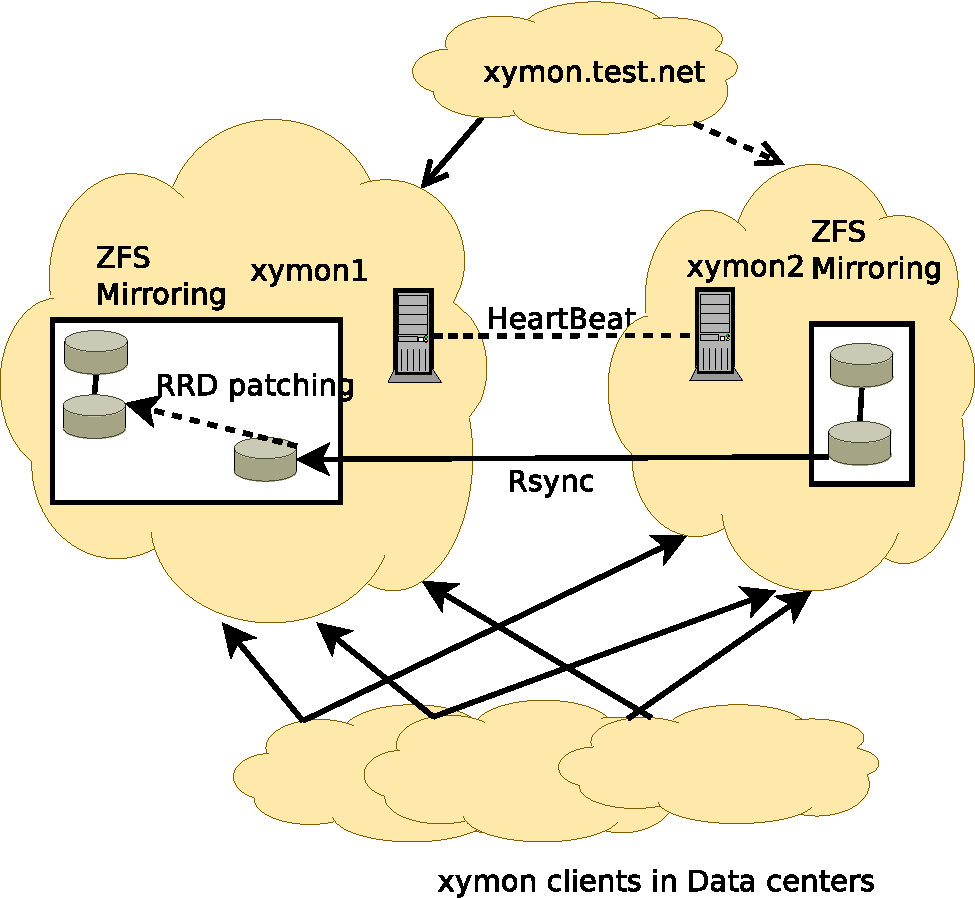
\includegraphics[scale=0.65]{dia/TwoNodeLooselyCpupledClusterWAN-RRDpatching.pdf}
\end{center}
\end{figure}

\item Extra remarks in the code \coderemark{Are displayed like this};
\begin{figure}[H]
\caption{Two Nodes Loosely Cupled Cluster WAN RRDpatching}
\label{TwoNodeLooselyCpupledClusterWAN-RRDpatching3}
\begin{center}
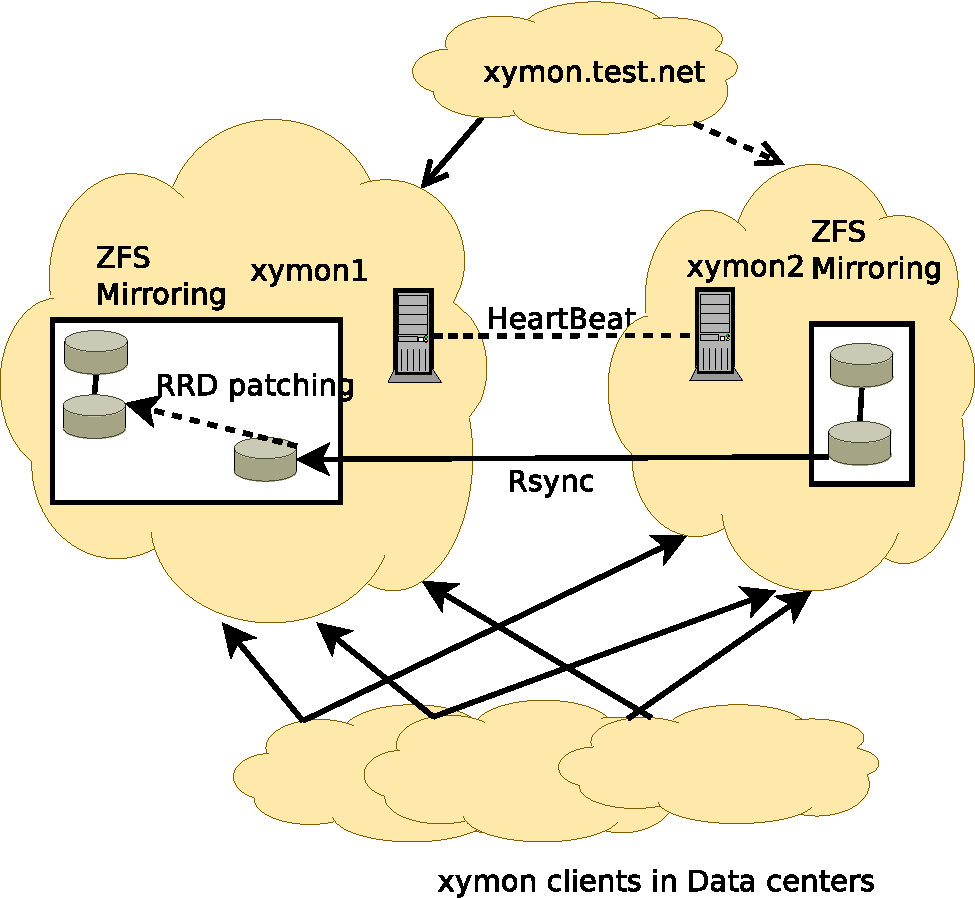
\includegraphics[scale=0.65]{dia/TwoNodeLooselyCpupledClusterWAN-RRDpatching.pdf}
\end{center}
\end{figure}

\item Longer remarks get a number -- \gocircle{1} -- with the explanation following;
\begin{figure}[H]
\caption{Two Nodes Loosely Cupled Cluster WAN RRDpatching}
\label{fig:TwoNodeLooselyCpupledClusterWAN-RRDpatching4}
\begin{center}
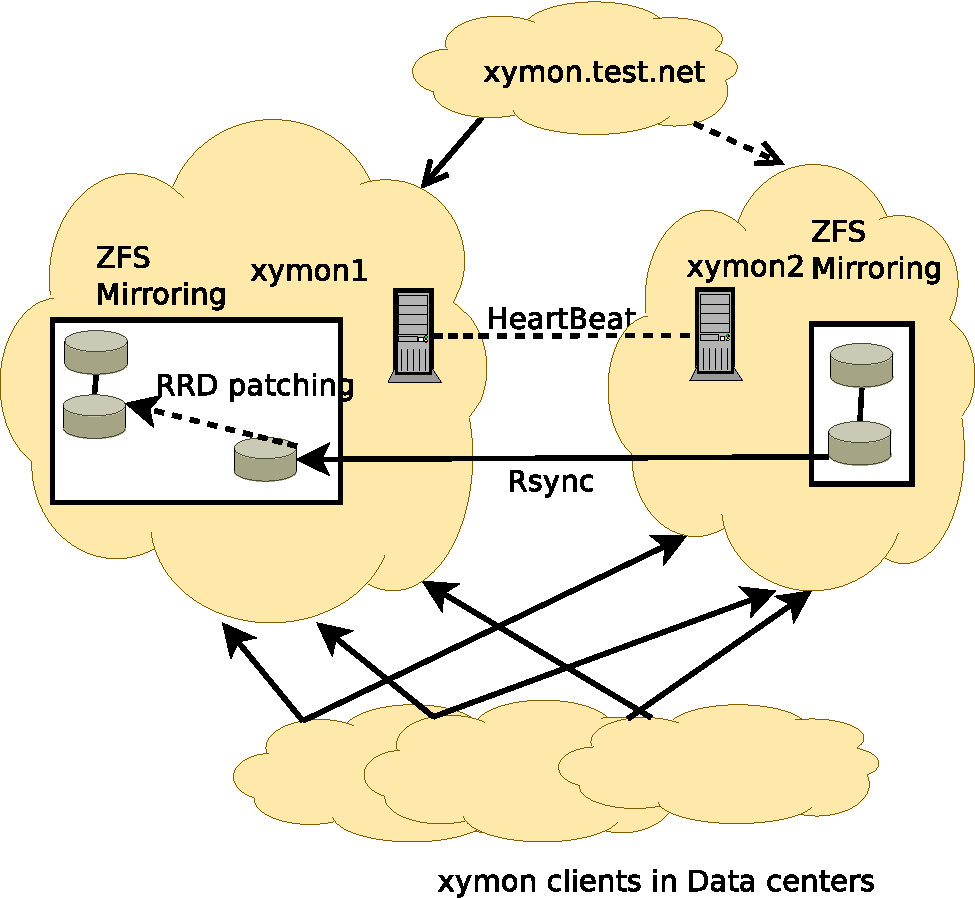
\includegraphics[scale=0.65]{dia/TwoNodeLooselyCpupledClusterWAN-RRDpatching.pdf}
\end{center}
\end{figure}

\item Line numbers are printed on the right side;
\begin{figure}[H]
\caption{Two Nodes Loosely Cupled Cluster WAN RRDpatching}
\label{fig:TwoNodeLooselyCpupledClusterWAN-RRDpatching5}
\begin{center}
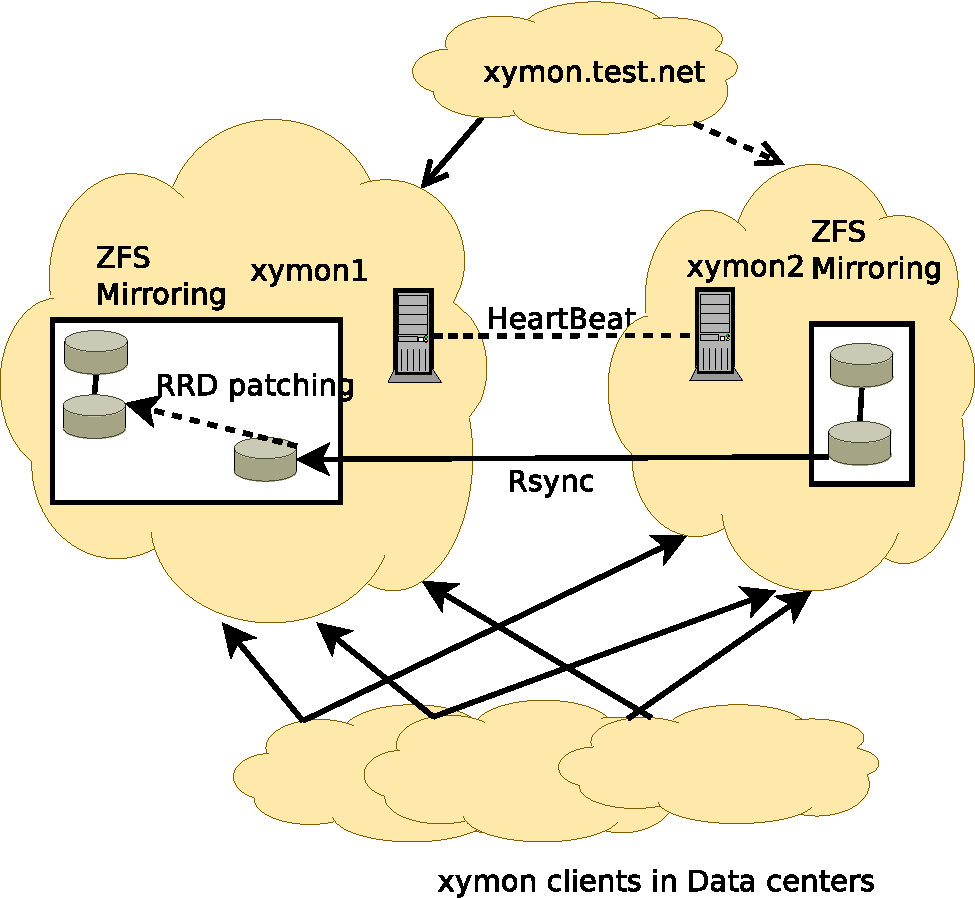
\includegraphics[scale=0.65]{dia/TwoNodeLooselyCpupledClusterWAN-RRDpatching.pdf}
\end{center}
\end{figure}

\item Shell examples use a \pr{} as prompt;
\begin{figure}[H]
\caption{Two Nodes Loosely Cupled Cluster WAN RRDpatching}
\label{fig:TwoNodeLooselyCpupledClusterWAN-RRDpatching6}
\begin{center}
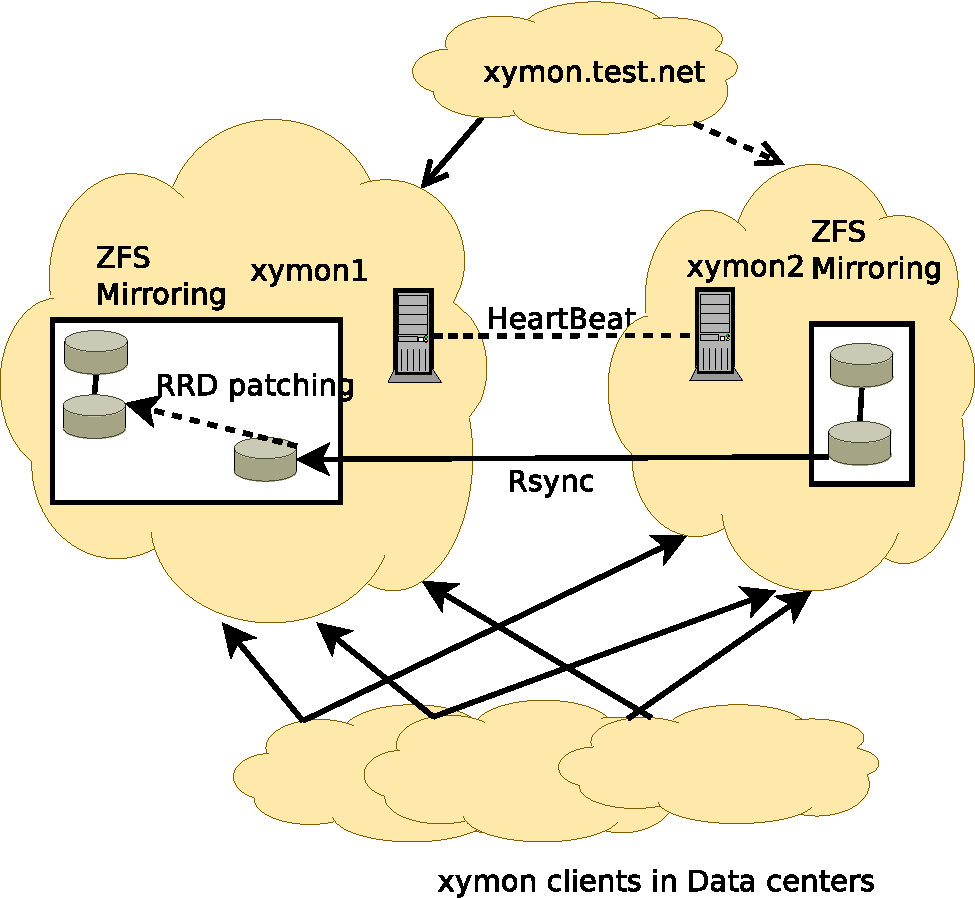
\includegraphics[scale=0.65]{dia/TwoNodeLooselyCpupledClusterWAN-RRDpatching.pdf}
\end{center}
\end{figure}

\item User entered text in shell examples \texttt{\user{is in bold}}, system responses
\begin{figure}[H]
\caption{Two Nodes Loosely Cupled Cluster WAN RRDpatching}
\label{fig:TwoNodeLooselyCpupledClusterWAN-RRDpatching7}
\begin{center}
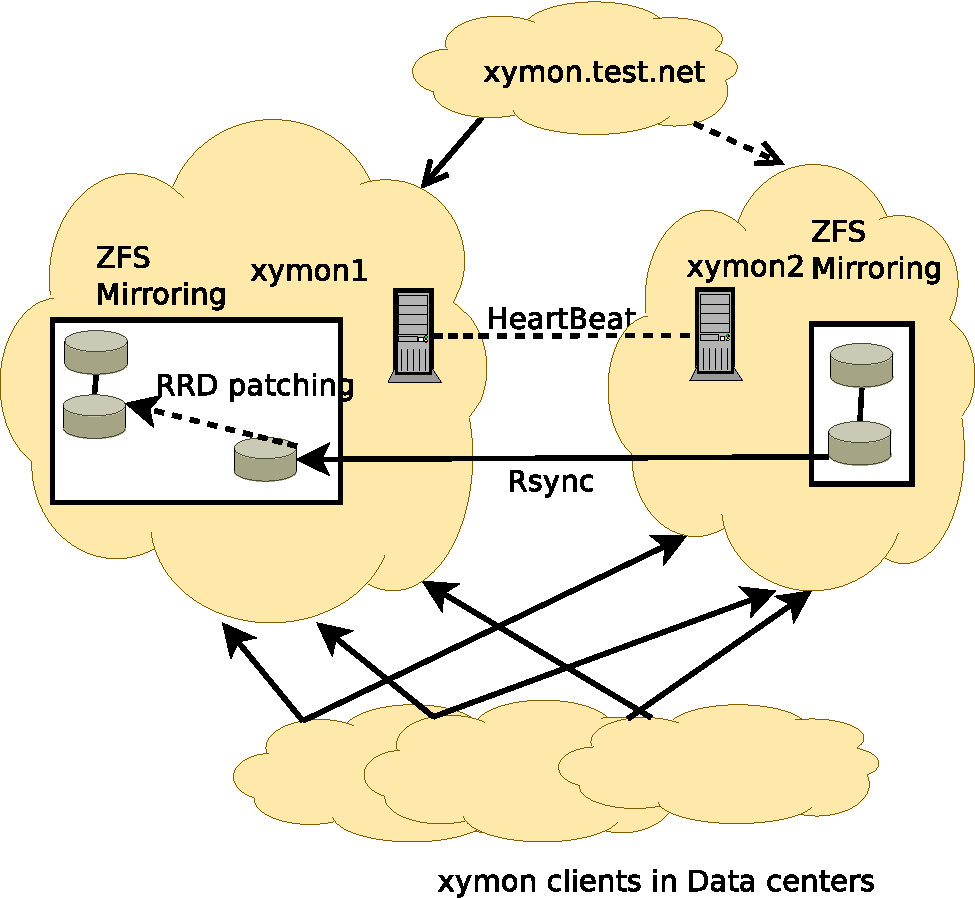
\includegraphics[scale=0.65]{dia/TwoNodeLooselyCpupledClusterWAN-RRDpatching.pdf}
\end{center}
\end{figure}

are in a \texttt{typewriter font};
\begin{figure}[H]
\caption{Two Nodes Loosely Cupled Cluster WAN RRDpatching}
\label{fig:TwoNodeLooselyCpupledClusterWAN-RRDpatching8}
\begin{center}
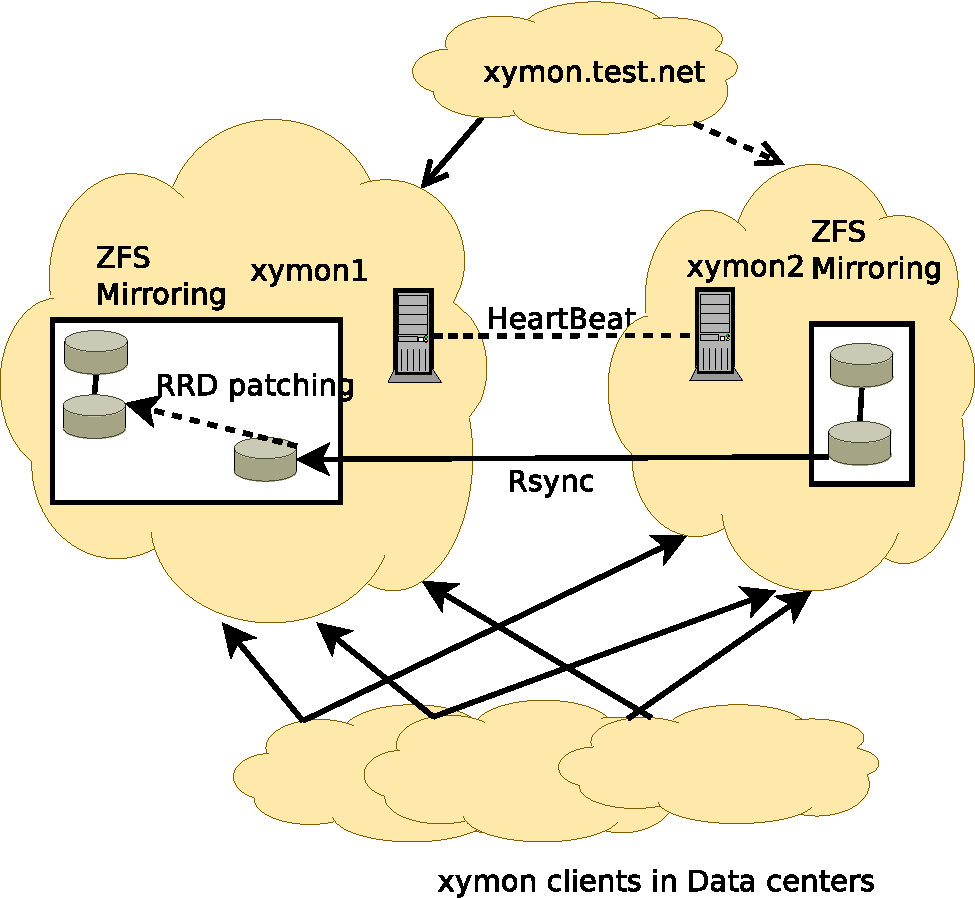
\includegraphics[scale=0.65]{dia/TwoNodeLooselyCpupledClusterWAN-RRDpatching.pdf}
\end{center}
\end{figure}

\item An emphasized paragraph is indented and has a vertical bar on the
left.
\begin{figure}[H]
\caption{Two Nodes Loosely Cupled Cluster WAN RRDpatching}
\label{fig:TwoNodeLooselyCpupledClusterWAN-RRDpatching}
\begin{center}
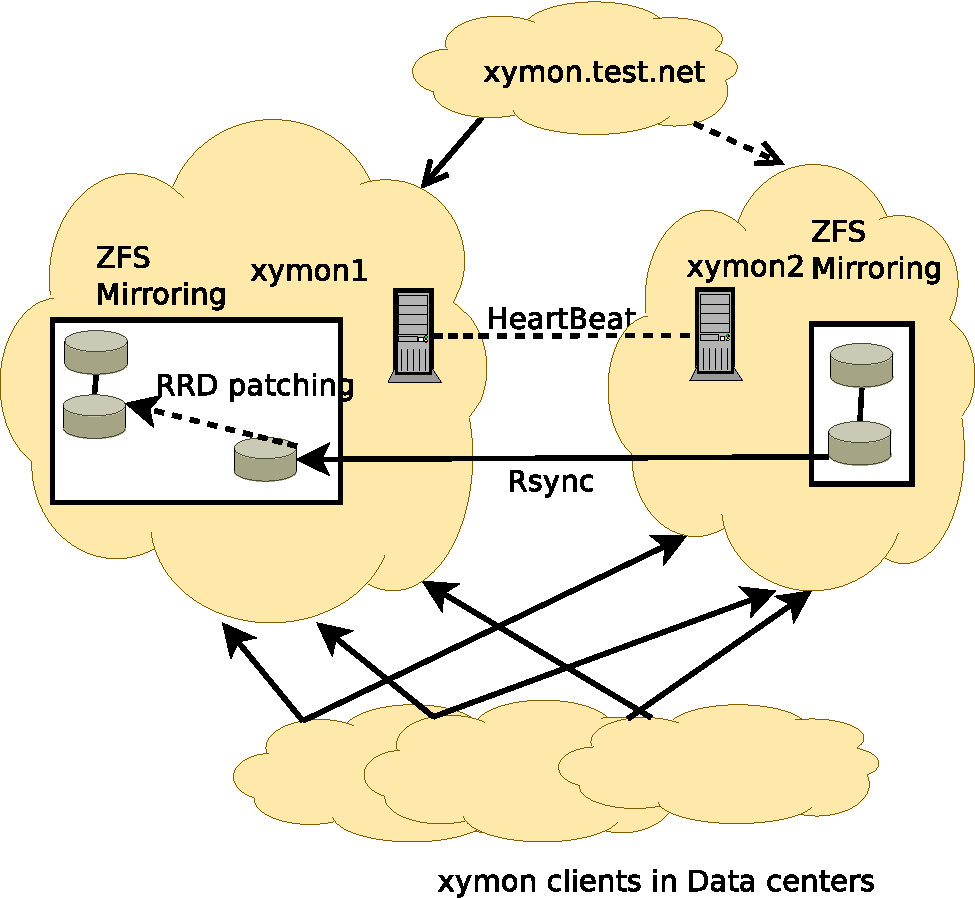
\includegraphics[scale=0.65]{dia/TwoNodeLooselyCpupledClusterWAN-RRDpatching.pdf}
\end{center}
\end{figure}

\end{itemize}

